\documentclass[conference]{IEEEtran}
\usepackage{graphicx}
\usepackage{float}
\usepackage{amsmath}
%\usepackage{cite}

\begin{document}

\title{Direction of Angle Estimation}

\author{\IEEEauthorblockN{Owen Sowatzke}
\IEEEauthorblockA{\textit{Electrical Engineering Department} \\
\textit{University of Arizona}\\
Tucson, USA \\
osowatzke@arizona.edu}}
\maketitle

\begin{abstract}
	Direction of arrival (DOA) estimation plays an integral role in radar, wireless communications, sonar, radio astronomy, and navigation \cite{doa_algorithms_raghu}. Specific algorithms for DOA estimation include beamforming, MVDR, MUSIC, improved MUSIC, Root Music, and ESPRIT \cite{doa_algorithms_raghu}. Following the work of Raghu and Kamari, this paper evaulates the performance of each of these direction of arrival algorithms operating on data from a uniform linear array. 
\end{abstract}

	\section{Background}
	
	Each of the direction of angle algorithms compared in this report operate on data collected with an antenna array. This report specifically examines data collected with a uniform linear array (ULA). A block diagram of a uniform linear array with $M$ antenna elements, receiving signals from $D$ sources is given by Raghu and Kamari in \cite{doa_algorithms_raghu}.
	
	\begin{figure}[H]
		\centerline{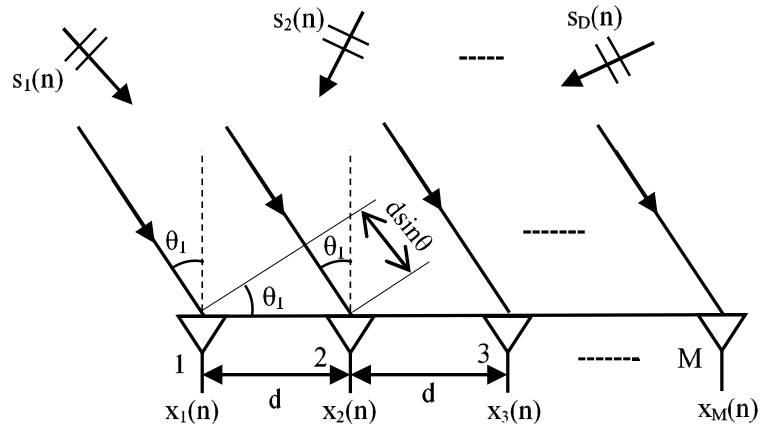
\includegraphics[width=0.5\textwidth]{uniform_linear_array.png}}
		\caption{Uniform Linear Array \cite{doa_algorithms_raghu}}
	\end{figure}
	
	As shown in the figure above, let $d$ be the distance between successive array elements, and $\beta$ be defined as $2\pi/\lambda$. Then if each of the source signals is given as $s_1(n),...,s_D(n)$, the signal received by m-th array element can be written as:
	%
	\begin{equation}
		\label{received_signal}
		\begin{split}
			x_m(n) &= s_1(n)e^{-j{\beta}d(m-1)\sin{\theta_1}} + \cdots\\
			&+ s_D(n)e^{-j{\beta}d(m-1)\sin{\theta_D}} + w_m(n)
		\end{split}
	\end{equation}
	%
	where $w_m(n)$ denotes the noise on the m-th element \cite{doa_algorithms_raghu}.
	
	Equation (\ref{received_signal}) can be rewritten in matrix form as follows:
	%
	\begin{equation}
		X = AS + W
	\end{equation}
	%
	where $X = \begin{bmatrix} x_1(n) & \cdots & x_n(n)\end{bmatrix}^T$ is the Mx1 received signal vector, $A$ is the MxD array steering matrix, $S = \begin{bmatrix} s_1(n) & \cdots & s_D(n)\end{bmatrix}^T$ is the Dx1 source signal vector, and $W = \begin{bmatrix} w_1(n) & \cdots & w_n(n)\end{bmatrix}^T$ is the Mx1 noise signal vector \cite{doa_algorithms_raghu}. The array steering matrix $A$ can be written as:
	%
	\begin{equation}
		A = \begin{bmatrix} a(\theta_1) & \cdots & a(\theta_D) \end{bmatrix}
	\end{equation}
	%
	where $a(\theta_i)$ represents the Mx1 array response for the source signal incident at angle $\theta_i$ and is defined in \cite{doa_algorithms_raghu} as:
	%	
	\begin{equation}
		\label{array_response_vector}
	 	a(\theta_i) = \begin{bmatrix} 1 & e^{-j{\beta}d\sin(\theta_i)} & \cdots & e^{-j{\beta}d(M-1)\sin(\theta_i)}\end{bmatrix}^T
	\end{equation}
	
		Each direction of arrival algorithm leverages spatial auto-correlation matrices $R_{xx}$ defined in \cite{doa_algorithms_raghu}  using the received signal vector $X$ as:
	%
	\begin{equation}
		R_{xx} = E[XX^H]
	\end{equation}
	%
	The expected value in the above equation is estimated using $K$ (a finite number) samples of the received signal vector $X$. The resulting spatial auto-correlation estimate ${R}_{xx}$ is given in \cite{doa_algorithms_raghu} as follows: 
	%
	\begin{equation}
		\label{spatial_matrix_estimate}
		\hat{R}_{xx} = \sum_{n=1}^{K}{X(n)X^H(n)}
	\end{equation}
	
	\section{Direction of Arrival Algorithms}
	
	\subsection{Beamforming}
	
		Beamforming uses the estimate of the spatial auto-correlation matrix $\hat{R}_{xx}$ defined in Equation (\ref{spatial_matrix_estimate}) to estimate the spatial spectrum $\hat{P}_{bf}(\theta)$ \cite{doa_algorithms_raghu}. The spatial spectrum estimate $\hat{P}_{bf}(\theta)$ is defined by
		%
		\begin{equation}
			\hat{P}_{bf}(\theta) = a^H(\theta)\hat{R}_{xx}a(\theta)
		\end{equation}
		%
		where $a(\theta)$ is the array response given in Equation (\ref{array_response_vector}).
		
		To estimate the direction of arrival, compute the spatial spectrum in discrete steps over a region of interest. Then, find the peaks of the spatial spectrum. The angles corresponding to the peaks are the directions of arrival for each source.
		
	\subsection{Capon/MVDR}
	
		The Capon algorithm seeks to minimize the power of received signals in all direction except for the look angle \cite{doa_algorithms_raghu}. The Capon spatial spectrum $\hat{P}_{capon}(\theta)$ is generated using  the spatial auto-correlation matrix estimated by Equation (\ref{spatial_matrix_estimate}). For each look angle $\theta$, the spatial spectrum is given by:
	%
	\begin{equation}
		\hat{P}_{capon}(\theta) = \frac{1}{a^H(\theta){\hat{R}_{xx}}^{-1}a(\theta)}
	\end{equation}
	%
	
		Similar to beamforming direction of arrival estimation, Capon direction of angle estimation requires generating the spatial spectrum in discrete steps over a region of interest. Then, this spectrum can be searched for peaks. The angle corresponding to the peaks are the directions of arrival for each source.
	
	\subsection{MUSIC}
	
		The Multiple Signal Classification (MUSIC) algorithm takes an eigen-decomposition of the spatial auto-correlation matrix to produce orthogonal signal and noise subspaces. The eigenvectors of the resulting noise subspace are used to generate a spatial spectrum which can be used to estimate the directions of arrival \cite{doa_algorithms_raghu}.
	
		To find the signal and noise subspaces, the spatial auto-correlation matrix must decomposed into its eigenvalues and eigenvectors:
	%
	\begin{equation}
		\hat{R}_{xx} = E{\Lambda}E^H
		\label{eigenvalue_decomposition_of_Rxx}
	\end{equation}
	%
	In the above equation, $\Lambda = \text{diag}\{\lambda_0,...,\lambda_{M-1}\}$ is the MxM diagonal eigenvalue matrix and $E=\{e_0,...,e_{M-1}\}$ is the MxM eigenvector matrix.
	
	Because there are $D$ sources and $M$ eigenvalues, the $N = M - D$ smallest eigenvalues should correspond to the noise subspace. Assume the eigenvalues are sorted in ascending order (i.e. $\lambda_0 < ... < \lambda_{M-1}$). Then, $\{\lambda_0,...,\lambda_{N-1}\}$ and their corresponding eigenvectors $\{e_0,...,e_{N-1}\}$ correspond to the noise subspace.
	
	The number of source signals $D$ is typically not known, but can be estimated using a variety of methods, which include AIC and MDL \cite{num_sources_est_salman}. Both of these algorithms require a flipped copy of the eigenvalues (i.e. $\lambda_0 > ... > \lambda_{M-1}$). Using the flipped eigenvalues, the number of sources estimated with AIC is given in \cite{num_sources_est_salman} as
	%
	\begin{equation}
		\begin{split}
		\hat{D} &= argmin_n\left(-2\log\left(\frac{\prod_{i=n}^{M-1}{{\lambda_i}^{\frac{1}{M-n}}}}{\frac{1}{M - n}\sum_{i=n}^{M-1}{\lambda_i}}\right)^{(M-n)K}\right. \\
		& \left. + 2n(2M - n) \vphantom{-2\log\left(\frac{\prod_{i=n}^{M-1}{{\lambda_i}^{\frac{1}{M-k}}}}{\frac{1}{M - n}\sum_{i=n}^{M-1}{\lambda_i}}\right)^{(M-n)K}} \right)
		\end{split}
		\label{AIC_num_sources}
	\end{equation}
	where $n$ is the index of each eigenvalue. Similarly, the number of sources estimated with MDL is given in \cite{num_sources_est_salman} as
	%
	\begin{equation}
		\begin{split}
		\hat{D} &= argmin_n\left(-\log\left(\frac{\prod_{i=n}^{M-1}{{\lambda_i}^{\frac{1}{M-n}}}}{\frac{1}{M - n}\sum_{i=n}^{M-1}{\lambda_i}}\right)^{(M-n)K}\right. \\
		& \left. + \frac{1}{2}n(2M - n)\log(K) \vphantom{-\log\left(\frac{\prod_{i=n}^{M-1}{{\lambda_i}^{\frac{1}{M-k}}}}{\frac{1}{M - n}\sum_{i=n}^{M-1}{\lambda_i}}\right)^{(M-n)K}} \right)
		\end{split}
		\label{MDL_num_sources}
	\end{equation}
	
		Using the estimated number of sources $\hat{D}$, the number of noise eigenvalues/eigenvectors is approximately $\hat{N} = M - \hat{D}$. Let $E_n = \{e_0,...,e_{N-1}\}$ be the MxN noise subspace. Then, the music spectrum is given in \cite{doa_algorithms_raghu} as
	%
	\begin{equation}
		\label{music_spectrum}
		\hat{P}_{music}(\theta) = \frac{1}{a^H(\theta)E_n{E_n}^Ha(\theta)}
	\end{equation}
	
		As was the case with the other direction direction of angle algorithms, the music spectrum must be generated in discrete steps of a region of interest and then searched for peaks. The angles corresponding peaks are the angles of arrival.
		
	\subsection{Improved-MUSIC}
	
		The MUSIC algorithm produces poor angle estimates when the source signals are correlated \cite{doa_algorithms_raghu}. The Improved-MUSIC algorithm overcomes this limitation. It starts by performing a conjugate reconstruction of the received signal vector X with the matrix J \cite{doa_algorithms_raghu}.
		%	
		\begin{equation}
			Y = JX^{*}
		\end{equation}
		%
		where J is defined is defined as follows:
		%
		\begin{equation}
			J = \begin{bmatrix}
				0 & 0 & \cdots & 0 & 1\\
				0 & 0 & \cdots & 1 & 0\\
				\vdots & \vdots & \ddots & \vdots & \vdots\\
				1 & 0 & \cdots & 0 & 0
			\end{bmatrix}
		\end{equation}
		
		Then, the spatial auto-correlation matrix of the received signal vector $X$ is computed using Equation (\ref{spatial_matrix_estimate}). The spatial auto-correlation matrix of the transformed received signal vector $Y$ is given in \cite{doa_algorithms_raghu} as
		%
		\begin{equation}
			\hat{R}_{yy} = \sum_{n=1}^{K}{Y(n)Y^H(n)}
		\end{equation}
		%
		A new spatial auto-correlation matrix with the same noise subspace can be generated following \cite{doa_algorithms_raghu} as follows:
		%
		\begin{equation}
			\hat{R} = \hat{R}_{xx} + \hat{R}_{yy}
		\end{equation} 
		
		Following the MUSIC algorithm with $\hat{R}$ in place of $\hat{R}_{xx}$, a spatial spectrum can be derived for the Improved-MUSIC algorithm. The spatial spectrum can then be searched for peaks. The angles corresponding to these peaks are the directions of arrival for each source.
			
	\subsection{Root-MUSIC}
		
		The Root-MUSIC algorithm involves finding the roots of a polynomial and selecting the roots which correspond to sources. In contrast to the other algorithms presented, it does not require computing and searching through the spatial spectrum for peaks.
		
		Similar to the MUSIC algorithm, the Root-MUSIC algorithm involves computing an estimate of the spatial auto-correlation matrix and then finding the eigenvalues which correspond to the noise subspace. The Root-MUSIC algorithm then evaluates where the denominator of the MUSIC spectrum given by Equation (\ref{music_spectrum}) is zero. According to \cite{root_music_ko}, the denominator of the music spectrum can be written in the following form:
		%
		\begin{equation}
			\setlength{\arraycolsep}{2pt}
			\renewcommand{\arraystretch}{0.8}
			\begin{bmatrix}z^0 & z^{-1} & \cdots & z^{-(M-1)}\end{bmatrix}\begin{bmatrix}c_{11} & c_{12} & \cdots & c_{1M}\\ c_{21} & c_{22} & \cdots & c_{2M}\\ \vdots & \vdots & \ddots & \vdots\\ c_{M1} & c_{M2} & \cdots & c_{MM}\end{bmatrix}\begin{bmatrix}z^0 \\ z^1 \\ \vdots \\ z^{M-1}\end{bmatrix}
		\end{equation}
		%
		where $z = e^{-j{\beta}\sin{\theta}}$ and each $c_{ij}$ term is an element of the matrix $C = E_{n}{E_{n}}^H$.
		
		After performing matrix multiplication, the resulting polynomial can be expressed in the following form:
		%
		\begin{equation}
			\label{root_music_summation}
			\sum_{i=1}^{M}{\sum_{j=1}^{M}{C_{ij}z^{-i+j}}}
		\end{equation}
		%
		Grouping like terms, Equation (\ref{root_music_summation}) can be further simplified to the form given in \cite{doa_algorithms_raghu}
		%
		\begin{equation}
			\label{root_music_summation_simplified}
		 	\sum_{i=-M+1}^{M-1}{c_iz^i}
		\end{equation}
		%
		where $c_i$ is the sum of the diagonal $i$ elements above the main diagonal.
		
		Equation (\ref{root_music_summation_simplified}) can be multiplied by $z^{M-1}$ to get a polynomial with only positive powers of $z$. Then, the $2(M-1)$ roots of the polynomial can be found. $M - 1$ of these roots lie inside the the unit circle. Of these roots, the $\hat{D}$ closest to the unit circle correspond to signal roots \cite{root_music_eskandari}. The direction of arrivals for each source is then given by \cite{doa_algorithms_raghu} as 
		%
		\begin{equation}
			\theta_i = -\sin^{-1}\left[\frac{\lambda}{2{\pi}d}\text{arg}(z_i)\right]
		\end{equation}
		%
		where $z_i$ is one of the roots near the unit circle.
		
	\subsection{ESPRIT}
		
		Estimation of Signal Parameters via Rotational Invariance Technique (ESPRIT) uses rotational invariance of the signal subspace to perform direction of angle estimation \cite{root_music_ko}. It starts by dividing the M-element antenna array into two identical subarrays as illustrated in \cite{doa_algorithms_raghu}.
		
		\begin{figure}[H]
			\centerline{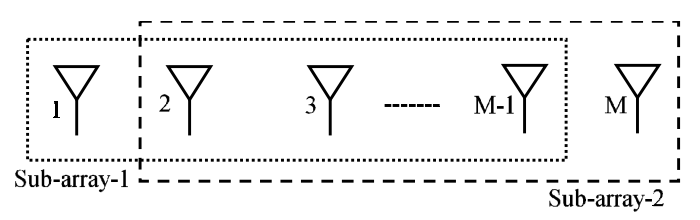
\includegraphics[width=0.5\textwidth]{esprit_doublets.png}}
			\caption{Antenna Array Divided into Two Subarrays \cite{doa_algorithms_raghu}}
			\label{esprit_subarrays}
		\end{figure}
		
		To perform the ESPRIT algorithm, capture $K$ samples of the received signal and estimate the spatial auto-correlation matrix using equation (\ref{spatial_matrix_estimate}). Then, perform an eigenvalue decomposition of the spatial auto-correlation matrix using equation (\ref{eigenvalue_decomposition_of_Rxx}). The output of the eigenvector decomposition will be an MxM diagonal matrix $\Lambda = \text{diag}\{\lambda_0, ..., \lambda_{M-1}\}$ and an MxM eigenvector matrix $E = \begin{bmatrix}e_0 & \cdots & e_{M-1}\end{bmatrix}$. 
		
		Next, estimate the number of sources $D$ using either equation (\ref{AIC_num_sources}) or equation (\ref{MDL_num_sources}). If the eigenvalues are sorted in descending order $\lambda_0 > \lambda_1 > \cdots > \lambda_{M-1}$, then the $D$ largest eigenvalues and their respective eigenvectors ($e_0, e_1, ..., e_{D-1}$) correspond to sources. These eigenvectors can be grouped into an MxD matrix $E_s = \begin{bmatrix} e_0 & \cdots e_{D-1} \end{bmatrix}$.
		
		$E_s$ can be further split into two submatrices $E_{s1}$ and $E_{s2}$ following to the array division shown in Fig. \ref{esprit_subarrays}. Specifically, $E_{s1}$ is the first $M-1$ rows of $E_s$, and $E_{s2}$ is the last $M-1$ rows of $E_s$. Next, compute the eigenvalue decomposition of the following combination of $E_{s1}$ and $E_{s2}$:
		
		\begin{equation}
			\begin{bmatrix}
				E_{s1}^H\\[6pt]
				E_{s2}^H
			\end{bmatrix}
			\begin{bmatrix}
				E_{s1} & E_{s2}
			\end{bmatrix}
			= V{\Lambda}V^H
		\end{equation}
		
		

		% angles corresponding of each signal root can be found by using the
		%The sum of the terms on the main diagonal will be weighted by $z^0$, the sum of the terms directly above the main diagonal will be weighted by $z^1$, and so on. The terms in the resulting polynomial will be weighted by powers of $z$ from $-(M-1)$ to $M-1$.
		
		%$C_ij$. jrh The terms on the main diagonal with all hav
		%this is the point at which the algorithms begin to differ.The MUSIC spectrum is then given by Equation (\ref{music_spectrum}). The denominator of the spectrum can be written in the following form:
		
	%\begin{equation}
	%	A = \begin{bmatrix}
	%		1 & 1 & \cdots & 1\\
	%		e^{j{\beta}d\sin{\theta_1}} & e^{j{\beta}d\sin{\theta_2}} & \cdots & e^{j{\beta}d\sin{\theta_D}} \\
	%		\vdots & \vdots & \ddots & \vdots\\
	%		e^{j{\beta}d(M-1)\sin{\theta_1}} & e^{j{\beta}d(M-1)\sin{\theta_2}} & \cdots & e^{j{\beta}d(M-1)\sin{\theta_D}}
	%	\end{bmatrix}
	%\end{equation}
	\bibliographystyle{IEEEtran}
	\bibliography{IEEEabrv,sources}
\end{document}